\subsubsection*{Mobile Application}
\subparagraph*{Events}
In order to better understand the system, it is necessary to identify the events that may occur, how the system will respond to the event, what caused the event and what type of event it is. For the remote client mobile application, the events that may occur are presented in table \ref{table:rc_app_events}.

\begin{table}[ht]
	\centering
	\resizebox{\columnwidth}{!}
	{
		\begin{tabular}{|m{3cm}|m{5cm}|m{2.4cm}|m{2.4cm}|}
			\hline
			\textbf{Event} & \textbf{System Response} & \textbf{Source} & \textbf{Type}\\
			\hline\hline
			Login & Show application main screen if successful & Operator & Asynchronous\\
			\hline
			
			Obtain geolocation & Request device geolocation & Mobile device & Asynchronous\\
			\hline
			
			App notification & Notifies the operator about the lamppost status & Remote Server & Asynchronous\\
			\hline
			
			Register operator & Add operator information to database & Operator & Asynchronous\\
			\hline
			
			Modify lamppost & Update lamppost information on database & Operator & Asynchronous\\
			\hline
			
			Register lamppost & Add lamppost information to database & Operator & Asynchronous\\
			\hline			
		\end{tabular}
	}
	\caption{Remote client events - mobile application.}
	\label{table:rc_app_events}
\end{table}

\subparagraph*{Use Cases}
The mobile application use cases diagram is represented in figure \ref{fig:UseCases_application}, showing that the main actors in the system are the operator, the database and the mobile device. The operator can perform operations such as login, logout, register, modify data about a lamppost and register newly installed posts that are installed, using, for this, the database (to obtain and record data) and the mobile device (to obtain the device location when registering a new post).

\begin{figure}[H]
	\centering
	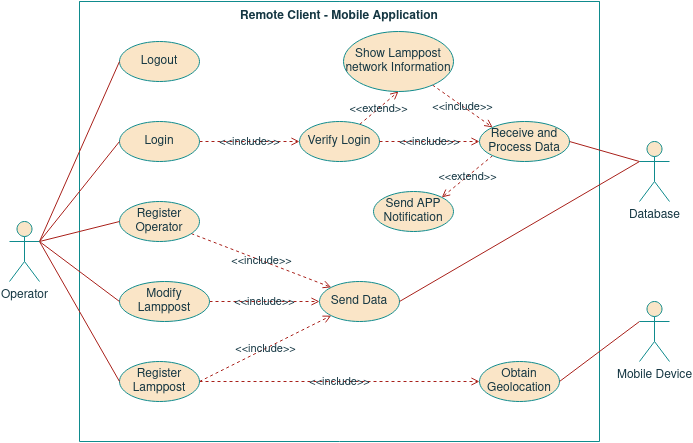
\includegraphics[width=0.85\textwidth]{06remote_system/AppSystem_UseCases}
	\caption{Remote System – Mobile Application Use Cases.}
	\label{fig:UseCases_application}
\end{figure}

\subparagraph*{State Chart}
In the figure \ref{fig:StateChart_application} is represented the state chart of the mobile application. It initiates with the system configuration, showing a home screen that allows the operator, the application user, to log into the system or register himself, if he doesn’t have login credentials. After a successful login, the system will show information about the lampposts associated to the logged in operator and he can do operations like register lampposts, modify lampposts information and logout of the system.

\begin{figure}[H]
	\centering
	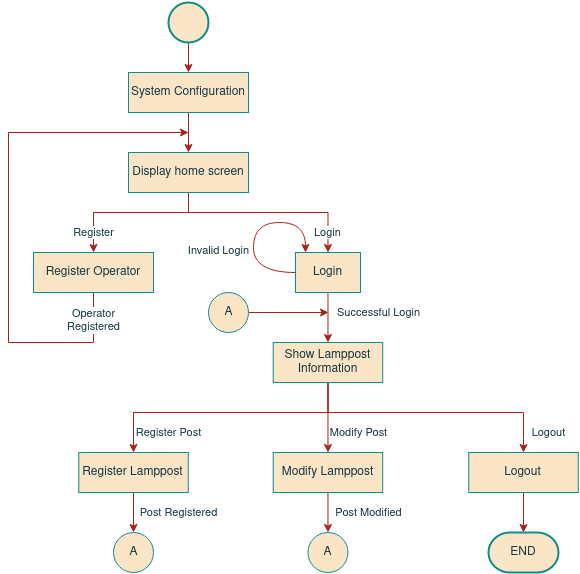
\includegraphics[width=.94\textwidth]{06remote_system/AppSystem_StateChart}
	\caption{Remote System – Mobile Application State Chart.}
	\label{fig:StateChart_application}
\end{figure}


\subparagraph*{Sequence Diagram}
In figure \ref{fig:SeqDiagram_WebSite} is represented the sequence diagram of the mobile application. Most of the actions are triggered by the operator, starting with the registration or login operations in the application. If the login is valid, information about the network of lampposts will be shown and, depending on the interaction with the operator, the application may have different execution flows: registration of a lamppost; changing information about a lamppost; verification of the existence of damaged posts, notifying the operator if so. If the login is invalid, the application returns an error to the operator.

\begin{figure}[H]
	\centering
	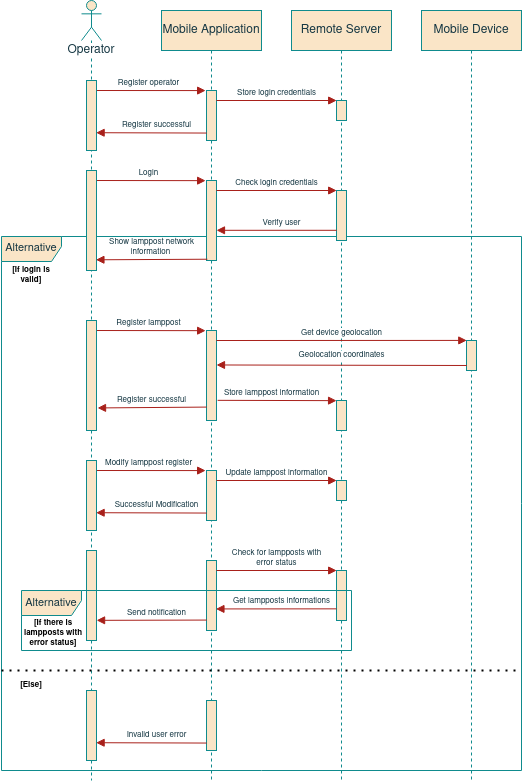
\includegraphics[width=0.90\textwidth]{06remote_system/AppSystem_SeqDiagram}
	\caption{Remote System – Mobile Application Sequence Diagram.}
	\label{fig:SeqDiagram_application}
\end{figure}
